\documentclass[tikz,border=2]{standalone}
\newcommand{\asd}{\alpha_s}
\newcommand{\afm}{\alpha_{\ell}}
\newcommand{\ald}{\alpha_{\ell d}}
\definecolor{RED}{HTML}{E41A1C}
\definecolor{BLUE}{HTML}{377EB8}
\definecolor{GREEN}{HTML}{4DAF4A}
\definecolor{ORANGE}{HTML}{FF7F00}
\usetikzlibrary{shadows,arrows,shapes,positioning,calc,backgrounds,fit,automata}
\begin{document}
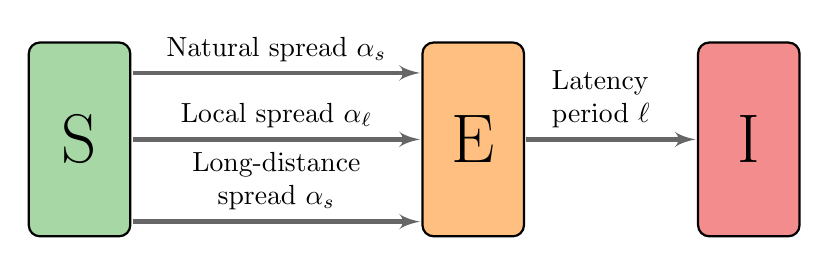
\begin{tikzpicture}
[auto, block/.style ={rectangle, draw=black, thick, text width=3em,
align=center, rounded corners, minimum height=7em,font=\Huge},
dedge/.style={ultra thick, black!60, >=latex', shorten >=.5pt, shorten <=.5pt}]
\node[block,fill=GREEN!50] (S) {S};
\node[block,fill=ORANGE!50] (E) at (5,0) {E};
\node[block,fill=RED!50] (I) at (8.5,0) {I};
\draw[->,dedge] ($(S.north east)+(0,-.4)$) -- ($(E.north west)+(0,-.4)$) 
node[midway,above,black] {Natural spread $\asd$};
\draw[->,dedge] (S) -- (E) 
node[midway,above,black] {Local spread $\afm$};
\draw[->,dedge] ($(S.south east)+(0,.2)$) -- ($(E.south west)+(0,.2)$) 
node[midway,above,black,text width=2.5cm,align=center] {Long-distance spread $\asd$};
\draw[->,dedge] (E) -- (I) node[midway,above,black] {\parbox{1.5cm}{Latency period~$\ell$}};

\end{tikzpicture}
\end{document}
